% Introdução

\documentclass[_ArquivoPrincipal.tex]{subfiles}

\begin{document}

%==================================================================================================
\section{Conceitos Iniciais} \label{CI}
%==================================================================================================

\textcolor{red}{Comentar brevemente alguns conceitos que irão ser utilizados: notação simbólica, indicial, delta de Kronecker, permutação de Levi-Cevita, integração por partes com o Teorema da divergência}

%==================================================================================================
\subsection{Integração Temporal} \label{MEFP-IntTemp}
%==================================================================================================

Como observado no equacionamento apresentado, há o surgimento de equações diferenciais com variações temporais. No entanto a determinação de uma expressão analítica que descreva o desenvolvimento dos parâmetros ao longo do tempo é de grande dificuldade, sendo necessário o desenvolvimento de métodos numéricos que representem adequadamente aos valores que a solução possui no tempo. Nesse cenário serão apresentados na presente seção alguns métodos de integração temporal baseados em diferenças finitas, sendo eles, o método por diferenças finitas adiantado (ou explícito), atrasado (ou implícito), central (ou semi-implícito), $\alpha$-generalizado e o método de Newmark.

Para se obter a taxa de variação temporal de uma propriedade qualquer $\phi$ ($\dot{\phi}=\partial\phi/\partial t$) a partir de uma abordagem de diferenças finitas adiantadas faz-se inicialmente uma expansão em séries de Taylor da mesma:

\begin{equation}
    \phi_{n+1}=\phi_n+\left.\frac{\partial\phi}{\partial t}\right|_n\Delta t+\frac{1}{2}\left.\frac{\partial^2\phi}{\partial t^2}\right|_n\Delta t^2+\cdots\text{,}\label{eq:TaylorAd}
\end{equation}

\noindent que, truncando a série no termo de primeira ordem, obtém-se:

\begin{equation}
    \dot{\phi}_n=\left.\frac{\partial\phi}{\partial t}\right|_n\approx\frac{\phi_{n+1}-\phi_n}{\Delta t}\text{.}
\end{equation}

\noindent Logo:

\begin{equation}
    \phi_{n+1}=\phi_n+\dot{\phi}_n\Delta t\text{.}
\end{equation}

Percebe-se que para se obter o valor posterior de uma propriedade segundo essa abordagem, é necessário conhecer somente valores presentes da mesma. Portanto o resultado desse integrador é obtido explicitamente. Além disso, como a série de Taylor foi truncada no termo de primeira ordem, então a ordem de precisão alcançada por esse integrador é $\script{O}(\Delta t)$.

Já nas diferenças atrasadas procede-se de forma semelhante, no entanto utilizando um intervalo de tempo $-\Delta t$, resultando em uma expansão em série de Taylor na forma:

\begin{equation}
    \phi_{n-1}=\phi_n-\left.\frac{\partial\phi}{\partial t}\right|_n\Delta t+\frac{1}{2}\left.\frac{\partial^2\phi}{\partial t^2}\right|_n\Delta t^2-\cdots\text{,}\label{eq:TaylorAt}
\end{equation}

\noindent que, ao truncar no termo de primeira ordem, obtém-se:

\begin{equation}
    \dot{\phi}_n=\frac{\phi_n-\phi_{n-1}}{\Delta t}\therefore
    \phi_n=\phi_{n-1}+\dot{\phi}_n\Delta t\text{,}
\end{equation}

\noindent que, ajustando os índices para um passo de tempo posterior, obtém-se:

\begin{equation}
    \phi_{n+1}=\phi_n+\dot{\phi}_{n+1}\Delta t\text{.}
\end{equation}

Portanto, pode-se observar que a determinação do valor posterior da propriedade depende de sua taxa de variação temporal nesse mesmo passo de tempo, sendo, assim, um procedimento implícito. E, da mesma forma que foi constatado no integrador explícito, esse possui uma ordem de precisão de $\script{O}(\Delta t)$.

Na sequência pode-se obter uma expressão que obtenha o valor da propriedade segundo uma abordagem de diferenças finitas centrais. Para isso subtrai-se \ref{eq:TaylorAt} de \ref{eq:TaylorAd}, obtendo-se:

\begin{equation}
    \phi_{n+1}-\phi_{n-1}=2\left.\frac{\partial\phi}{\partial t}\right|_n\Delta t+\frac{1}{3}\left.\frac{\partial^3\phi}{\partial t^3}\right|_n\Delta t^3+\cdots\text{,}\label{eq:TaylorCen}
\end{equation}

Como o termo de segunda ordem foi anulado, então pode-se realizar o truncamento no termo de primeira ordem sem perder a precisão obtida na segunda ordem. Assim, obtém-se que:

\begin{equation}
    \dot{\phi}_n=\left.\frac{\partial\phi}{\partial t}\right|_n\approx\frac{\phi_{n+1}-\phi_{n-1}}{2\Delta t}\text{.}
\end{equation}

\noindent Logo:

\begin{equation}
    \phi_{n+1}=\phi_{n-1}+2\dot{\phi}_n\Delta t\text{,}
\end{equation}

Também pode-se somar as equações \ref{eq:TaylorAd} e \ref{eq:TaylorAt} e fazer o truncamento no termo de primeira ordem, onde obtém-se que:

\begin{equation}
    \phi_n=\frac{\phi_{n+1}+\phi_{n-1}}{2}\text{.}
\end{equation}

Assim, trocando-se os índices $n-1\to n$ e $n\to n+1/2$ e tomando $\Delta t\to\Delta t/2$, tem-se que:

\begin{equation}
    \phi_{n+1}=\phi_n+\frac{\dot{\phi}_{n+1}+\dot{\phi}_n}{2}\Delta t\text{,}
\end{equation}

Essa solução pode ser entendida como a média entre as soluções das diferenças adiantadas com as diferenças atrasadas, possuindo uma precisão na ordem de $\script{O}(\Delta t^2)$. A Figura \ref{fig:DifFin} apresenta graficamente a interpretação das diferenças finitas adiantadas, atrasadas e centrais.

\begin{figure}[h]
    \centering
    \caption{Interpretação gráfica das diferenças finitas:}
    \begin{subfigure}{0.32\textwidth}
    \includegraphics[width=\linewidth]{Figuras/DifAd.pdf}
    \caption{Adiantadas.}
    \end{subfigure}
    \begin{subfigure}{0.32\textwidth}
    \includegraphics[width=\linewidth]{Figuras/DifAt.pdf}
    \caption{Atrasadas.}
    \end{subfigure}
    \begin{subfigure}{0.32\textwidth}
    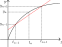
\includegraphics[width=\linewidth]{Figuras/DifCen.pdf}
    \caption{Centrais.}
    \end{subfigure}
    \\Fonte: Autoria Própria (\the\year).
    \label{fig:DifFin}
\end{figure}

\textcolor{red}{Talvez comentar também sobre o $\alpha$-generalizado \cite{chung1993time}}

Por fim, o método de Newmark apresenta-se como uma generalização do método das diferenças finitas centrais, inserindo dois parâmetros livres ($\beta$ e $\gamma$) que podem ser calibrados em função do problema estudado. Nesse sentido pode-se obter valores como posições ($\mathbf{y}$) e velocidades ($\dot{\mathbf{y}}$) como \textcolor{red}{(REFERÊNCIAS)}:

\begin{subequations}
    \begin{equation}
        \mathbf{y}_{n+1}=\mathbf{y}_n+\dot{\mathbf{y}}_n\Delta t+\left(\left(\frac{1}{2}-\beta\right)\Ddot{\mathbf{y}}_n+\beta\Ddot{\mathbf{y}}_{n+1}\right)\Delta t^2\text{,}
    \end{equation}
    \begin{equation}
        \dot{\mathbf{y}}_{n+1}=\dot{\mathbf{y}}_n+\left((1-\gamma)\Ddot{\mathbf{y}}_n+\gamma\Ddot{\mathbf{y}}_{n+1}\right)\Delta t\text{.}
    \end{equation}
\end{subequations}

Verifica-se que caso $\beta=1/4$ e $\gamma=1/2$ a aproximação de Newmark recai em um caso específico igual ao das diferenças centrais.

\textcolor{red}{(Comentar sobre estabilidade dos integradores)}

%==================================================================================================
\subsection{Integração numérica} \label{MEFP-IntNum}
%==================================================================================================

\textcolor{red}{Comentar sobre a integração por quadratura de Gauss e de Hammer}

\end{document}